
The elastic cross section of the deuteron is described by the charge ($G_C$), magnetic ($G_M$), and quadrupole ($G_Q$) form factors. In order to access all three form factors, measurements are needed for both polarized and unpolarized cross sections. 

In the unpolarized case, the cross section is determined by
\begin{equation}
\frac{d\sigma}{d\Omega} = \left. \frac{d\sigma}{d\Omega}\right\vert_{NS}\left[A(Q^2)  + B(Q^2)\tan^2\frac{\theta}{2}  \right],
\end{equation}
where $A$ and $B$ are related to the charge ($G_C$), magnetic ($G_M$), and quadrupole ($G_Q$) form factors by
\begin{equation}
A=G_C^2(Q^2)+\frac{8}{9} \eta ^2 G_Q^2 + \frac{2}{3} \eta G_M^2(Q^2),
\end{equation}
\begin{equation}
B=\frac{4}{3}\eta (1+\eta )G_M^2(Q^2).
\end{equation}
The $A$ and $B$ form factors have been measured to high precision by many experiments, as shown in Fig.~\ref{ab-ff}

\begin{figure}
\begin{center}
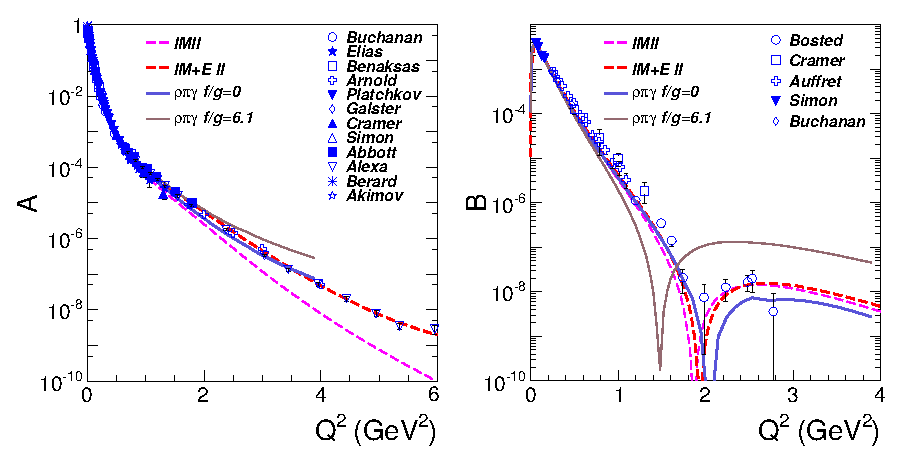
\includegraphics{figs/ab-ff.eps} 
\caption{\label{ab-ff}World data on the unpolarized deuteron form factors $A$ and $B$~\cite{Holt:2012gg}.}
\end{center}
\end{figure}

In order to separate out all three form factors, a measurement of the tensor analyzing powers is also needed. Although a number of tensor analyzing powers are available, $T_{20}$ has proven to be the most informative and has been studied more indepth than the others. This analyzing power is defined by
\begin{equation}
T_{20} = -\frac{\frac{8}{9}\eta^2 G^2_Q + \frac{8}{3} \eta G_C G_q + \frac{2}{3} \eta G_M^2\left[\frac{1}{2} + (1 + \eta) \tan^2(\theta / 2) \right]}{\sqrt{2} [A + B\tan^2(\theta / 2)]},
\end{equation}
where $\eta=Q^2/4M^2$, and can be measured by knowing either the initial or final polarization state. With a measurements of $A$, $B$, and $T_{20}$, each of the three deuteron form factors can be extracted.

\begin{figure}
\begin{center}
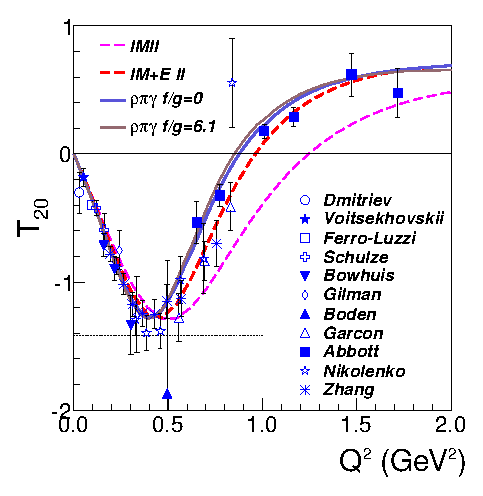
\includegraphics{figs/t20_data.eps} 
\caption{\label{t20-world}Existing world data on the tensor analyzing power $T_{20}$~\cite{Holt:2012gg}.}
\end{center}
\end{figure}

As shown in Fig.~\ref{t20-world}, the world data for $T_{20}$ is far less well-measured than $A$ and $B$. There are systematic discrepancies present between the different datasets, with measurements from JLab coming out less negative than those from Bates and VEPP-3 at higher $Q^2>0.5$~GeV$^2$, which affects model calculations particularly for determining $G_C$~\cite{Gilman:2001yh}.  Additionally, only a single experiment has been done for large $Q^2>1$~GeV$^2$~\cite{Abbott:2000fg}, where more data needs to be taken in order to confirm our present understanding of $T_{20}$.

An ideal measurement of $T_{20}$ would be taken over a large range of $Q^2$, which could use the lower $Q^2<0.4$~GeV$^2$ results to make sure that systematic uncertainties are well understood while simultaneously measuring the region of current discrepancies ($Q^2\approx0.75$~GeV$^2$) and extending to larger four-momentum transfer to confirm the single measurement taken at $Q^2>1$~GeV$^2$. By utilizing the same time-frame and kinematics that will be used to determine $A_{zz}$, we propose such a measurement.